% ======================================================================
% capitulos/linea2/capitulo7.tex
% ----------------------------------------------------------------------
% LÍNEA CE02 — Evidencia CE0212: Prototipo navegable validado
% ======================================================================
\section{Sección 2: Prototipo Navegable}
\label{chap:ce02-prototipo}

Esta sección corresponde a la evidencia \textbf{CE0212 — Prototipo navegable
validado}. El prototipo permitió validar con los usuarios la disposición de la
información y el flujo de trabajo \emph{antes} de construir el sistema definitivo, y
fue la base de las observaciones recogidas en el acta de la
\cref{sec:ce02-validacion}.

% ======================================================================
\subsection{Fidelidad y alcance}

Se construyó un prototipo interactivo de \textbf{fidelidad media} (clicable, con datos
de ejemplo) como aplicación web independiente en HTML, CSS y JavaScript, sin conexión
a un backend. Cubre las pantallas principales de los roles internos y una simulación
de la conversación del cliente por WhatsApp. Permite cambiar de rol desde el menú
lateral y recorrer el flujo real: venta $\rightarrow$ aprobación $\rightarrow$
coordinación $\rightarrow$ instalación $\rightarrow$ cobranza y corte.

\begin{table}[htbp]
\centering
\caption{Ficha del prototipo.}
\label{tab:ce02-ficha-proto}
\small
\begin{tabularx}{\textwidth}{L{3.5cm}X}
\toprule
Tipo & Prototipo de fidelidad media, navegable \\
Tecnología & HTML5, CSS3 y JavaScript (sin backend) \\
Pantallas & 10 pantallas principales + flujo de navegación \\
Roles cubiertos & Administrador (gerente/ingeniero), vendedor de campo, técnico y cliente (WhatsApp) \\
Validación & Sesión de revisión con usuarios de WISP (\cref{tab:ce02-acta}) \\
Enlace / repositorio & \rule{7cm}{0.4pt} \emph{(completar con la URL del prototipo publicado)} \\
\bottomrule
\end{tabularx}
\end{table}

% ======================================================================
\subsection{Flujo de navegación}

El diagrama resume cómo se conectan las pantallas y cómo la confirmación de una
instalación o un corte disparan la comunicación con el cliente.

\begin{figure}[htbp]
\centering
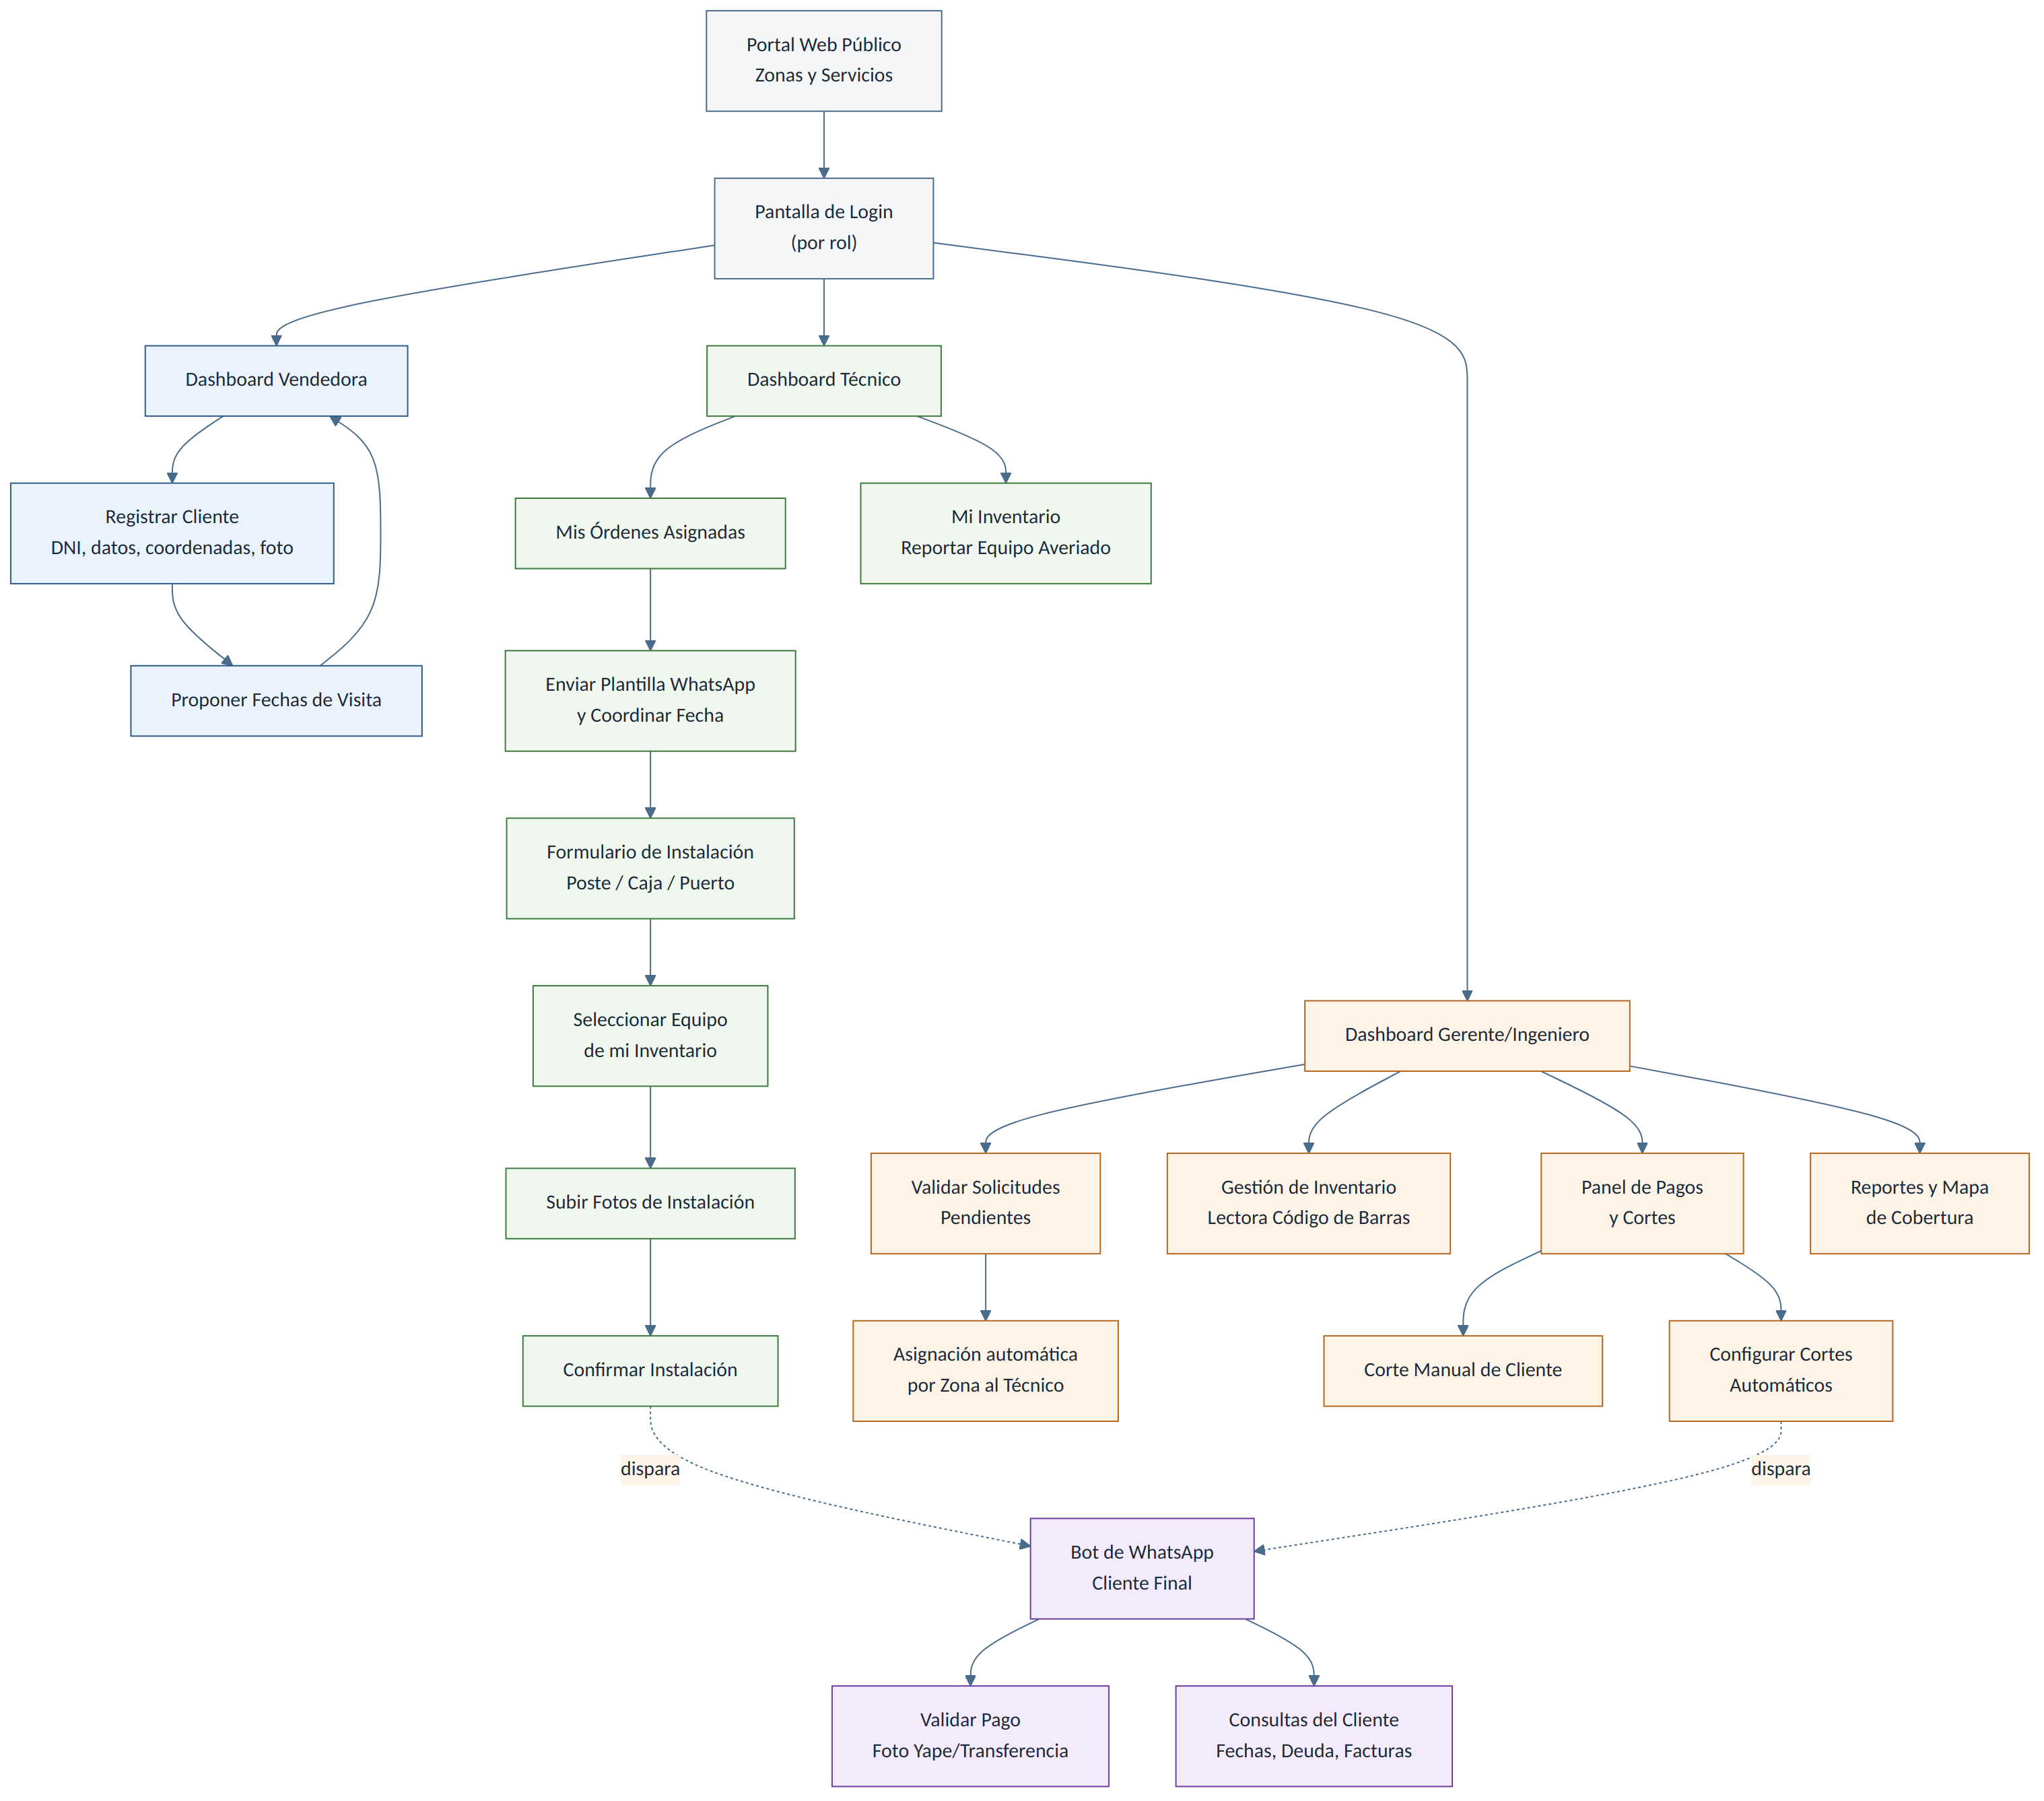
\includegraphics[width=\textwidth,height=0.42\textheight,keepaspectratio]{linea2/flujo_navegacion.png}
\caption{Flujo de navegación entre pantallas por rol.}
\label{fig:ce02-flujo}
\end{figure}

% ======================================================================
\subsection{Pantallas principales}

\newcommand{\pantalla}[3]{%
\begin{minipage}[t]{0.48\textwidth}\centering
\includegraphics[width=\linewidth,height=5.2cm,keepaspectratio]{linea2/#1}
\captionof{figure}{#2}\label{fig:ce02-#1}
\vspace{2pt}{\footnotesize\itshape #3}
\end{minipage}}

\begin{center}
\pantalla{proto_portal.png}{Portal público.}{Zonas de cobertura y planes, sin autenticación (RF-01, RF-02).}\hfill
\pantalla{proto_panel_vendedora.png}{Panel del vendedor.}{Solicitudes registradas y su estado.}
\end{center}
\begin{center}
\pantalla{proto_registro_cliente.png}{Registro de cliente.}{Datos, GPS y fotos de la vivienda (RF-05 a RF-08).}\hfill
\pantalla{proto_dashboard_tecnico.png}{Panel del técnico.}{Órdenes de su zona e inventario (RF-12).}
\end{center}
\begin{center}
\pantalla{proto_coordinar_visita.png}{Coordinar visita.}{Plantilla de WhatsApp para acordar la fecha (RF-13, RF-14).}\hfill
\pantalla{proto_registrar_instalacion.png}{Registrar instalación.}{Caja NAP, borne y equipo (RF-15 a RF-22).}
\end{center}
\begin{center}
\pantalla{proto_panel_gerencia.png}{Panel de gerencia.}{Indicadores y validación de ventas (RF-09 a RF-11).}\hfill
\pantalla{proto_inventario.png}{Inventario y lectora.}{Registro de equipos por código (RF-24 a RF-26).}
\end{center}
\begin{center}
\pantalla{proto_pagos_cortes.png}{Pagos y cortes.}{Estado de cuenta y corte manual o automático (RF-29 a RF-35).}\hfill
\pantalla{proto_bot_whatsapp.png}{Bot de WhatsApp.}{Simulación de validación de pago y consulta (RF-39 a RF-46).}
\end{center}

% ======================================================================
\subsection{Resultados de la validación}

\begin{table}[H]
\centering
\caption{Observaciones del prototipo y cómo se incorporaron al producto.}
\label{tab:ce02-obs-proto}
\small
\begin{tabularx}{\textwidth}{L{2.6cm}XL{3.8cm}}
\toprule
\textbf{Usuario} & \textbf{Observación} & \textbf{Incorporación} \\
\midrule
Vendedor & Capturar la ubicación por GPS y no escribirla. & RF-06; app móvil con \texttt{expo-location}. \\
Técnico & Ver la caja NAP como mapa visual de bornes. & RF-18; detalle de caja en la app y el panel. \\
Administrador & Mostrar de inmediato el dato escaneado para corregirlo. & RF-24; pantalla \texttt{escanear-equipo}. \\
Técnico & El técnico no debe imponer la fecha: solo la coordina con el cliente. & RF-13, RF-14 (pendientes). \\
Cliente / gerencia & Consultar la cuenta sin esperar al bot. & RF-44 a RF-46 resueltos con la App del cliente. \\
\bottomrule
\end{tabularx}
\end{table}

\begin{upeubox}{Del prototipo al producto}
El prototipo validó el flujo; el producto construido (\cref{chap:ce02-arquitectura})
lo implementa en un panel web (React) para administración y atención, y en una app
móvil (Expo) con tres espacios: técnico, vendedor y cliente. Las pantallas de
coordinación de visita y del bot con IA quedaron como trabajo pendiente del
semestre~2.
\end{upeubox}
